\clearpage
\chapter{Lexical analyzer for C language using Lex tool}

\section{Aim}
To design and implement a lexical analyzer for given C language using lex tool. The lexical analyzer should ignore redundant spaces, tabs and new lines.

\section{Algorithm}

\begin{figure}[H]
	\centering
	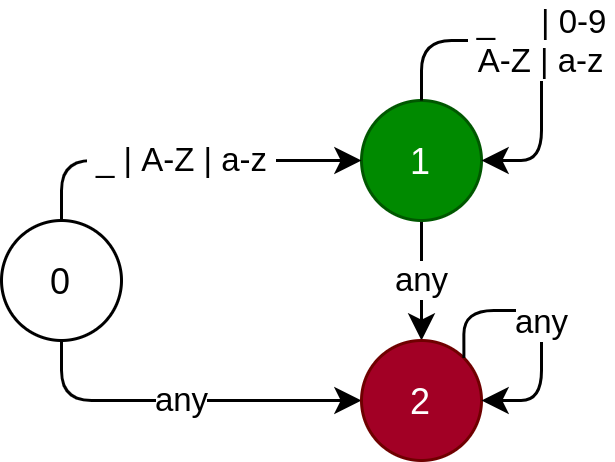
\includegraphics[height=2.5in]{../EXP1/identifier.png}
	\caption{Finite Automaton to detect an identifier.}
\end{figure}

\begin{figure}[H]
	\centering
	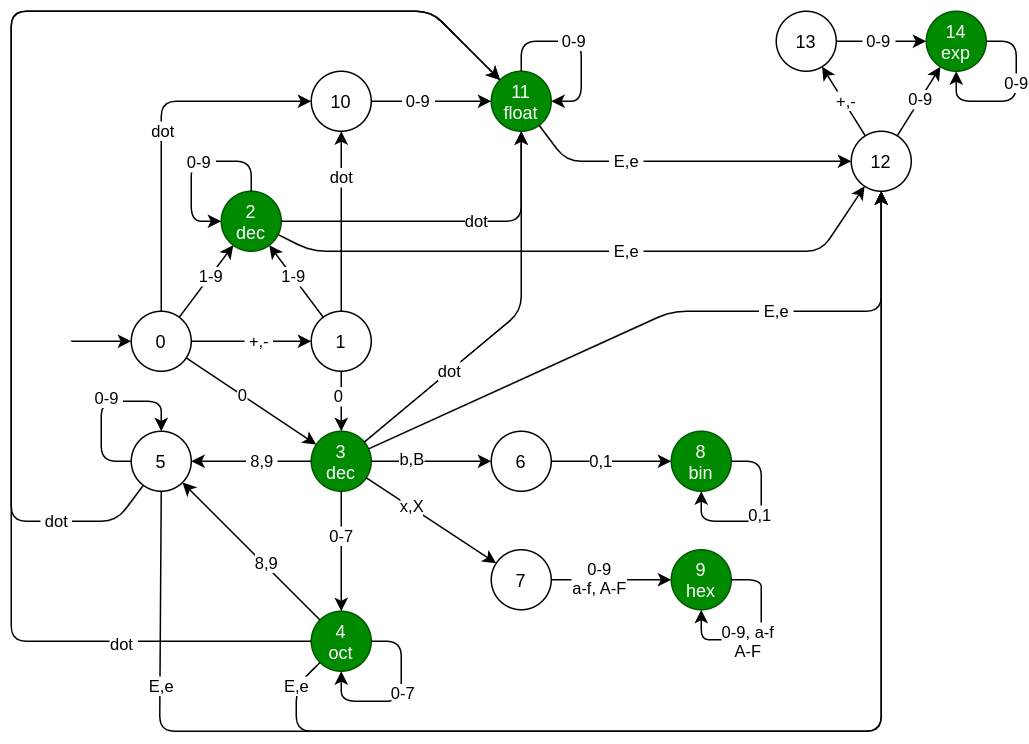
\includegraphics[width=\textwidth]{../EXP1/numerals.png}
	\caption{Finite Automaton to detect an numeral type.}
\end{figure}


\begin{figure}[H]
	\centering
	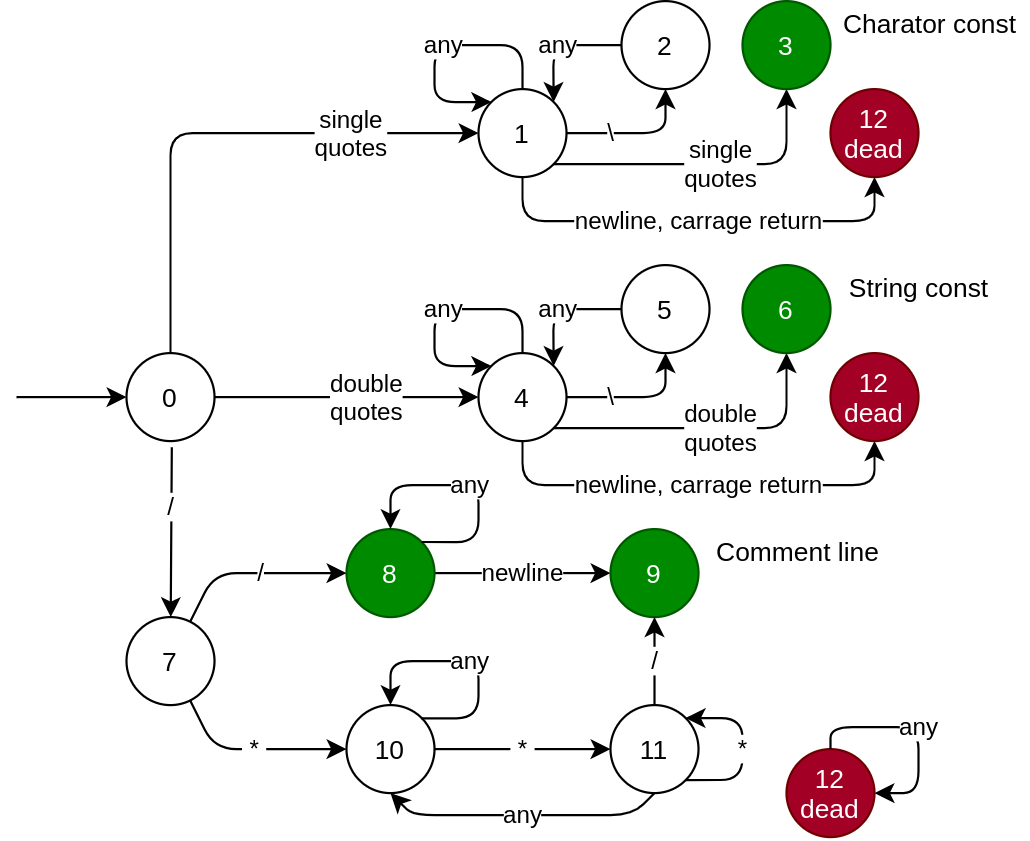
\includegraphics[width=\textwidth]{../EXP1/char-stream.png}
	\caption{Finite Automaton to detect comments, string/char literl and escape sequence}
\end{figure}


\section{C-Program}
Header file \textbf{stack.h} to stimulate stack.
\lstinputlisting[style=CStyle]{../EXP2/stack.h}

\vspace{0.5cm}
Header file \textbf{definition.h} holds various subroutines and constants that aid to analyze keywords and identifiers. The lex tool detects identifers. A table is cross checked to detect keywords.
\lstinputlisting[style=Cstyle]{../EXP2/definition.h}

\vspace{0.5cm}
Lex file \textbf{CLexical.l} initiates and scans lexemes.
\lstinputlisting[style=Cstyle]{../EXP2/CLexical.l}



\section{Output}
C program used for testing \textbf{sample.c}.
\lstinputlisting[style=CStyle]{../EXP2/sample.c}


\vspace{0.5cm}
Compiling lex file
\begin{lstlisting}[style=Terminal]
	$ lex CLexical.l
	$ gcc lex.yy.c
	$ ./a.out sample.c
\end{lstlisting}

\vspace{0.5cm}
Lexical analyser output
\lstinputlisting[style=plain]{../EXP2/sample_out.txt}

\section{Result}
The Lexicial analyser is stimulated successfully and the output is verified.